% ------ headers globales -------------
\documentclass[11pt, a4paper, twoside]{article}
\usepackage{header}
\usepackage{config}
% -------------------------------------
\begin{document}

% -- Carátula --
\clearpage{\pagestyle{empty}% parametros para la caratula (caratula.sty)

\materia{Sistemas Operativos}
%\submateria{}
\titulo{Trabajo Práctico 3}
\subtitulo{Algoritmos en sistemas distribuidos}
%\subtitulo{Escape en Sistemas}
\fecha{13 de noviembre de 2014}
\integrante{Rodriguez, Pedro}{197/12}{pedro3110.jim@gmail.com}
\integrante{Benegas, Gonzalo Segundo}{958/12}{gsbenegas@gmail.com}
\integrante{Barrios, Leandro Ezequiel}{404/11}{ezequiel.barrios@gmail.com}
%\grupo{Grupo ??}

\maketitle
}

%-- Índice --
\clearpage{%
  \pagestyle{empty}\tableofcontents%
  \vspace{3cm}%
  \cleardoublepage%
}
%-- A partir de aquí, pongo el contador de páginas en 1 --
\setcounter{page}{1}

\index{Introducción}
\section{Introducción}
En el presente trabajo práctico empleamos técnicas de programación paralela. En particular, nos centramos
en el diseño y la implementación de un servidor que a través del uso de múltiples hilos de ejecución
(\texttt{multithreading}) se encarga de atender concurrentemente las peticiones a distintos clientes. Esto
lo logramos siguiendo el modelo de $workers$ propuesto por la cátedra en el enunciado del TP.

En el TP se nos propone resolver el problema de coordinar adecuadamente la evacuación de un edificio. En el
modelo provisto por la cátedra, contamos con un sistema que procesa los pedidos de los clientes de forma
secuencial. Y nuestro objetivo es usar técnicas de multiprogramación para procesar estos pedidos de forma
paralela. En nuestro modelo, los clientes son personas que están en un espacio rectangular dividido en
metros cuadrados. Cada persona está en algún metro cuadrado y cada baldosa tiene un límite predefinido en
cuanto a la cantidad de personas que pueden estar en ese espacio al mismo tiempo.

\newpage
\index{Desarrollo}
\section{Desarrollo}
Para implementar el \texttt{servermulti} nos basamos en el código de \texttt{servermono} provisto por la
cátedra. Las tareas que tuvimos que realizar para lograr la administración paralela de los pedidos por
parte de los clientes fueron:
\begin{enumerate}
\item Para cada cliente que pida entrar a nuestro sistema, largamos un $thread$ que se encargue de la
  comunicación entre \texttt{servermulti} y dicho cliente. Todos estos $threads$ comparten el acceso a un
  mismo bloque de memoria. Es esta la razón por la cuál tuvimos que emplear varios \texttt{mutex} y \texttt{variables de condición}
  para administrar correctamente el acceso a estas posiciones de memoria.
\\ \textit{Observación}: se utilizan variables de condición en vez de semáforos porque son los mecanismos con los que cuenta la especificación de \texttt{pthreads}.

\begin{figure}[H]
\centering
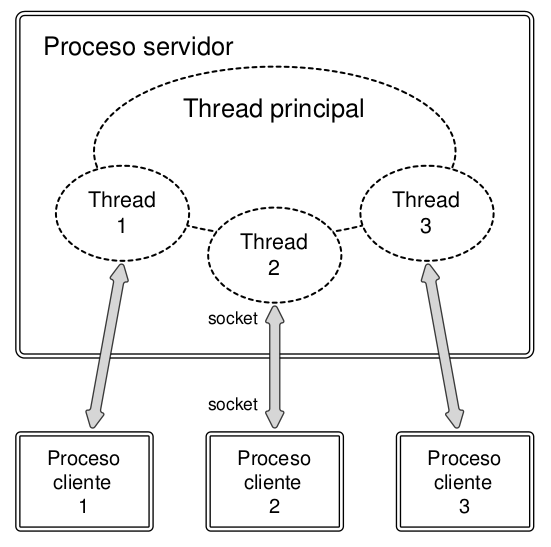
\includegraphics[scale=0.66]{esquema-workers.png}
\caption{Croquis del nuevo diseño propuesto}
\end{figure}



\item Cada vez que un cliente pide desplazarse de una casilla del aula a otra, manejar correctamente el
  acceso a dichas celdas y actualizar correctamente las variables globales que determinan el estado actual
  del sistema en cada instante.
\item Manejar correctamente la salida definitiva del edificio de las personas que ya están afuera del mismo.
  Para esto tuvimos que tener cuidado con,  para cada persona que logra salir de la habitación, determinar
  si hay algún rescatista libre en ese momento para ponerle la máscara y así poder posteriormente (cuando
  hayan llegado otras cuatro personas junto a ella) salir definitivamente del edificio y salvarse. Si no lo
  hay, la persona tiene que esperar a que llegue un rescatista y le ponga una máscara antes de poder salvarse
  definitivamente (podrían haber más de cinco personas fuera del aula pero esperando a que lleguen rescatistas
  para que le pongan la máscara y recién ahí, cuando hayan cinco personas con máscara, puedan salir).

\end{enumerate}

\par Un problema importante que nos surgió fue el de evitar $deadlock$ cuando dos $a$ y $b$ que están en las
casillas $A$ y $B$ piden acceso a $B$ y $A$ respectivamente. Para arreglar este potencial problema, lo que
hicimos fue considerar un orden especial en el tomado de los \texttt{mutex}. Consideramos un \textbf{orden global}, de acuerdo al índice de la posición en la matriz, primero por fila y después por columna. En general, de esta forma prevenimos cualquier deadlock ocasionado por una situación de espera circular. Como no se cumple una de las condiciones de Coffman, podemos garantizar que el sistema está libre de deadlock.

\par Para manejar correctamente la espera de los rescatistas utilizamos dos variables: una para contabilizar
la cantidad de personas fuera del edificio \textbf{con máscara} y por otro lado la cantidad de personas
fuera del edificio pero \textbf{esperando máscara}.

\par Cuando testeamos nuestro código, vimos que el tiempo que tardaban los rescatistas en ponerle la máscara
a cada una de las personas era muy corto. Entonces, para que la existencia de rescatistas tenga sentido y su
existencia sea considerable cuando corremos nuestro \texttt{servermulti}, agregamos un tiempo de tardanza
que tarda cada rescatista tarde en colocar una máscara a una persona.

\subsection{Escalamiento}
%% Analizar solución entregada
%% Proponer mejoras de software y hardware
\centerbf{Cantidad de Puertos}

La limitación más evidente es que, con la implementación actual, cada thread mantendría abierta una conexión local ocupando un puerto de origen distinto (todas con destino al puerto \texttt{5555}. Dado que el número de puerto es un \texttt{unsigned short}, la cantidad máxima de puertos es 65536. Por lo tanto, en estas condiciones estaríamos lejos de poder atender 1000000 de clientes.

Verificamos la afirmación del párrafo anterior mediante la ejecución del comando \texttt{netstat -tupaln}. Se adjunta a continuación un output de ejemplo, para 30 clientes.

\lstinputlisting[language=bash,basicstyle=\scriptsize,emph={tcp},keywordstyle=\color{blue},stringstyle=\color{red},tabsize=2,caption=netstat -tupaln]{netstat.txt}

En un sistema en donde los clientes se conecten desde distintas IPS, este factor no representaría necesariamente una limitación, ya que cada cliente utilizaría el puerto que tuviera disponible (el servidor siempre utiliza el puerto 5555).

\centerbf{Recursos del sistema}
Ya que la creación de un thread consume cierta cantidad de recursos, una decisión posible es tener un \textit{pool} de threads creados al inicializar el servidor.

Una primera consideración es que, al crecer la cantidad threads, se les otorga \emph{quantum} de procesador con cada vez menor frecuencia. Dada la urgencia de la evacuación, el \emph{turnaround} puede ser muy alto para ser factible. La persona podría estar esperando mucho tiempo sin recibir respuesta por parte del servidor. La mejora propuesta, en este caso, es de hardware, y consiste en aumentar la cantidad de recursos.

El segundo aspecto a tener en cuenta, es la cantidad de memoria que ocupa cada \emph{Thread}. En un acercamiento experimental lanzamos el servidor con 1000 clientes, y verificamos la cantidad de memoria ocupada del sistema operativo antes de lanzar la prueba (1GB), y luego de que se abrieran todas las conexiones (4GB). La diferencia, 3GB, dividido 1000, la cantidad de clientes, da una cantidad de memoria de aproximadamente 3MB por thread.

Hay que tener en cuenta que en el análisis anterior se tomó la memoria del servidor, y la que ocupa cada cliente que se conecta, ya que todo el test corrió localmente. Intentamos realizar el test en forma remota, y por alguna razón (a pesar de que los clientes abrían la conexión correctamente) no logramos hacer que ninguno de los clientes se muevan.

Intentamos entonces realizar un monitoreo exhaustivo de la memoria ocupada por el proceso \texttt{server\_multi}, junto con sus threads, a través de \texttt{ps}, \texttt{top / htop}, \texttt{valgrind}, pero al parecer el sistema operativo no brinda fácilmente esa información, ya que en todos los casos la memoria del proceso particular se mantenía constante luego de haber abierto cientos de conexiones (y por consiguiente, cientos de threads).

Bajo las consideraciones anteriores, asumimos entonces que necesitaríamos un máximo aproximado de 3MB por thread. En un servidor con 1 millón de clientes conectados al mismo tiempo, esto se traduce en 3TB de memoria, una cantidad que, si bien es inmensa, sigue siendo razonable en un entorno de \texttt{supercomputadora}.

Asumiendo que no estamos utilizando una supercomputadora, podemos pensar en una solución basada en un \texttt{pool de threads}. Esto es, a grandes rasgos, una estructura (ejemplo, un arreglo) de threads de cantidad fija o dinámica. A su vez, se mantiene una cola de tareas a ejecutar, las cuales se van asignando a los threads del \texttt{pool} a medida que estos se van liberando. Este modelo se complementa bien con nuestra implementación, ya que se basa en que cada thread del pool es un worker, lo mismo que ya ocurre con nuestra versión del servidor multithread. La versión más básica de un pool de threads mantiene siempre una cantidad fija de threads. Esto puede ser perjudicial, por ejemplo, si hay muy pocos threads efectivamente en uso (ej, pocas conexiones) estamos desperdiciando memoria y recursos para mantener muchos threads que no se están usando. Si por el contrario hay demasiados clientes, vamos a tener muchos threads ocupados constantemente. Suponiendo que la cantidad de clientes pueda variar inesperadamente, o que respete cierto patrón, otra posibilidad es utilizar una cantidad de threads dinámica, de forma tal que el servidor pueda realizar un autoescalamiento en la medida que le lleguen muchos clientes (y se mantengan en el tiempo), y que en el caso de que la cantidad de clientes descienda drásticamente pueda liberar los recursos utilizados por los threads que se encuentran disponibles.

% considerar memoria de tener threads: ver http://stackoverflow.com/questions/7235934/pthreads-high-memory-usage

% la idea del thread pool: http://en.wikipedia.org/wiki/Thread_pool_pattern


\newpage
\index{Conclusión}
\section{Conclusión}

%% implementacion interesante - variable d condicion - concepto nuevo: pthreads - peligrosidad paralelismo
%% buenas practicas para este ecosistema, cada vez más presente en la industria - primer acercamiento a
%% la programación de un servidor - muy interesante - todas las mejoras que se le pueden hacer a un servidor
%% y como esto impacta en el cliente (que solemos ser nosotros)

Primero que nada, tenemos que decir que el trabajo práctico nos pareció muy entretenido. La implementación del modelo propuesto por la cátedra fue para nosotros un desafío ya que implicó el aprendizaje y manejo básico de herramientas importantes para un programador, como los \texttt{pthreads} o \texttt{variables de condición}.

Durante el desarrollo de la implementación, nos encontramos frente a los problemas comunes que se pueden
presentar en la programación de sistemas paralelizados. En estos casos, tuvimos que aplicar las buenas prácticas de programación en este tipo de sistemas, como por ejemplo la protección de variables compartidas y/o memoria compartida.

Además, nos pareció muy estimulante acercarnos por primera vez a lo que es la programación de un servidor, y ver
de primera mano cómo un servidor puede y debe ser tuneado para soportar una cantidad grande de pedidos por parte de una gran cantidad de clientes.

\end{document}
